\documentclass{article}
%Para imagenes
\usepackage{graphicx}
\usepackage{float}
\usepackage{enumitem} % Paquete para personalizar listas
\usepackage[margin=2cm]{geometry} % Ajusta todos los márgenes a 2 centímetros
\usepackage{indentfirst} % Este paquete fuerza la sangría del párrafo en la primera línea
\setlength{\parindent}{1cm} % Ajusta la sangría de los párrafos a 1 cm




\begin{document}
	\begin{titlepage}
		\centering
		{\bfseries\LARGE Universidad de Granada\par}
		\vspace{1cm}
		{\scshape\Large Facultad de Ingeniería Informática \par}
		\vspace{2cm}
		{\scshape\Huge Practica 1: Patrones de diseño \par}
		\begin{figure}[h]
            	\centering
            	
\includegraphics[width=0.75\textwidth]{logo_UGR.jpg}
            	\label{fig:portada}
            \end{figure}
		{\itshape\Large DS: Grupo 1.7\par}
		\vfill
			{\Large  Emanuel Giraldo Herrera\par}
			{\Large  Thomas Lang \par}
			{\Large  Timur Sorokin \par}
			{\Large  Alejando Iborra Morán \par}
		\vfill
		{\Large (2023-2024) \par}
	\end{titlepage}
	
	\section{Ejercicio 1 (Java)}
	\subsection{Análisis}
	\noindent Se trata de realizar una simulación de carreras de bicicletas con las siguientes características:
	\begin{itemize}
		\item \textbf{Bicicleta}\\
		Cada bicicleta tiene un identificador. Existen dos tipos de bicicletas:
		\begin{itemize}
			\item Carretera
			\item Montaña
		\end{itemize}
		

			\item \textbf{Carrera}\\
			No se conoce el número de bicicletas antes de que empiece la carrera. Además, para cada tipo de bicicleta existe su tipo de carrera con las siguientes peculiaridades:
			\begin{itemize}
				\item Carretera\\
				Antes de finalizar 10\% bicicletas abandonan la carrera
				\item Montaña\\
				Antes de finalizar 20\% bicicletas abandonan la carrera.
				\item Hebras\\
				Se utilizarán las hebras para la simulación simultanea de varias carreras
		\end{itemize}
\end{itemize}

\noindent Finalmente, los objetivos que se buscan son aplicar dos patrones de diseño: Factoría Abstracta y Factoría método.


\subsection{UML}
Antes de realizar la implementación primero hemos de plantear el diagrama UML que relacione las entidades del problema y refleje sus interacciones.
\begin{figure}[h]
	\centering
	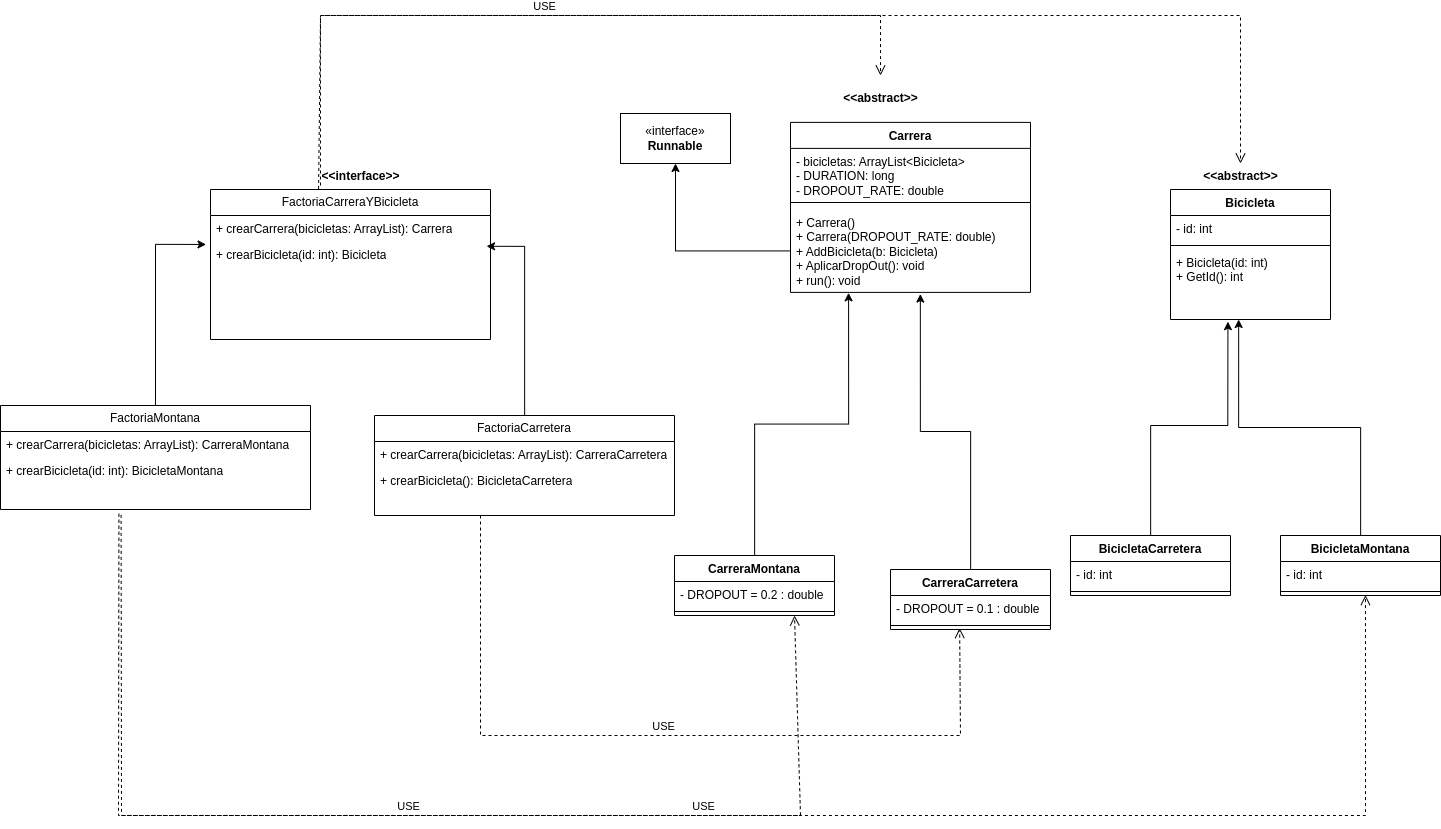
\includegraphics[width=1\textwidth]{DS_ej1.drawio.png}
	\caption{Factoría Abstracta}
	\label{fig:factoria_abstracta}
\end{figure}

\newpage
\begin{figure}[h]
	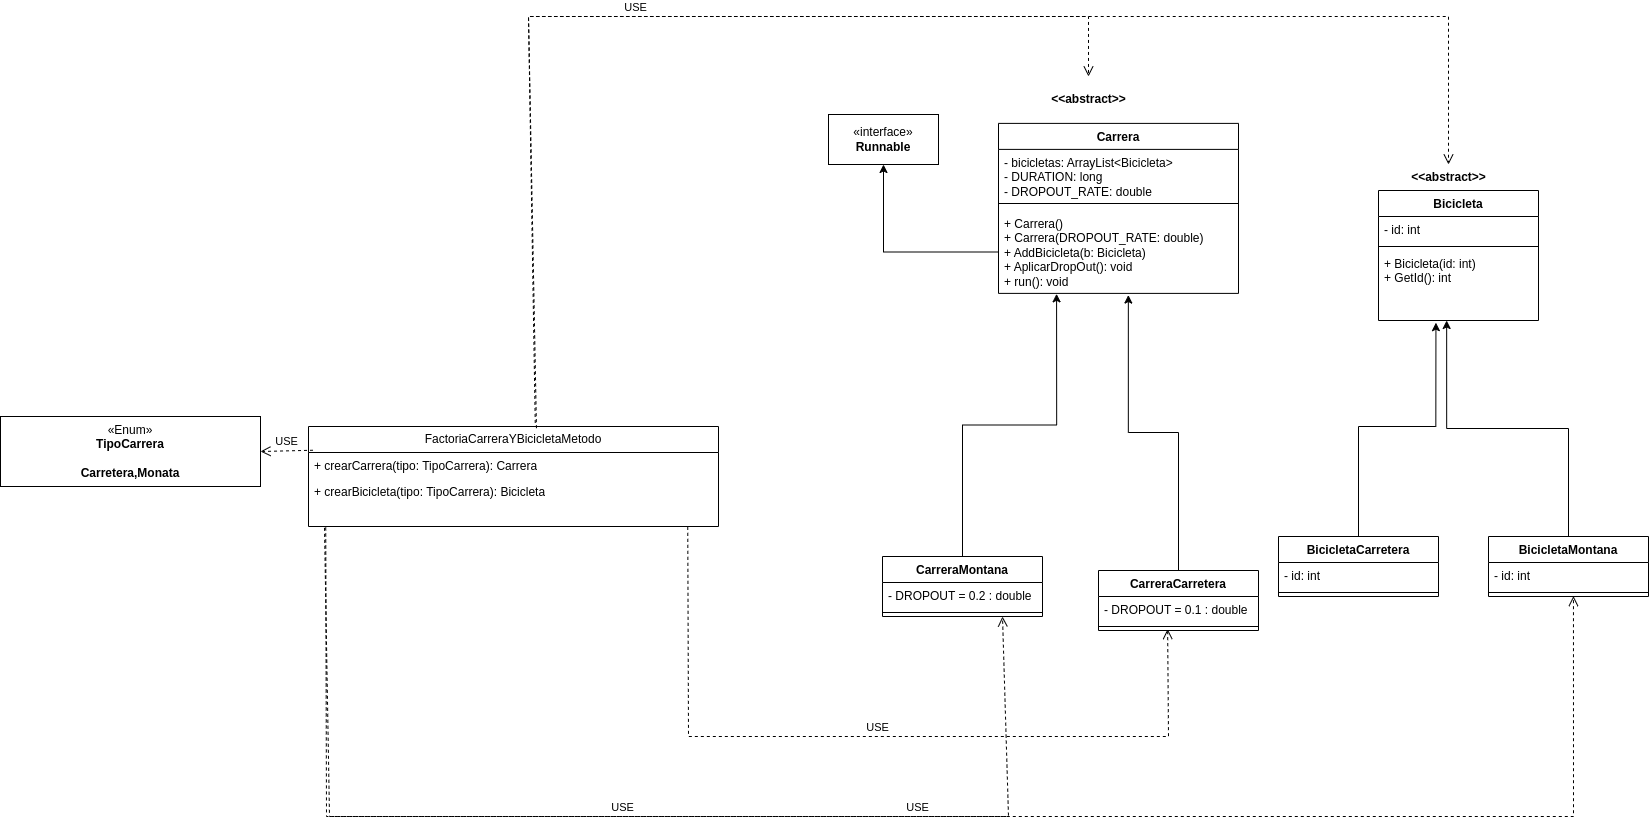
\includegraphics[width=1\textwidth]{factoria_metodo.png}
	\caption{Factoría Método}
	\label{fig:factoria_metodo}
\end{figure}

\subsection{Factoría Abstracta}
Se trata de un patrón creacional que define una interfaz para crear objetos relacionados sin especificar las clases concretas de esos objetos. Así conseguimos que el código cliente pueda instanciar los objetos sin conocer sus tipos concretos. Esto nos permite desacoplar las implementaciones concretas del código cliente. \\

En nuestro problema tenemos dos entidades básicas que son \textit{Bicicleta} y \textit{Carrera}. Hemos visto durante el análisis que existe una relación entre estas  dos clases, es decir, en una \textit{Carrera} compiten las \textit{Bicicletas}. También vimos que ambas entidades pueden ser de dos tipos: \textit{carretera} y \textit{montaña}. Cada uno de ellos con sus características \textit{concretas}. 
Entonces, tenemos que en una \textit{Carrera de montaña} participan \textit{Bicicletas de montaña}. Y en una \textit{Carrera de carretera} participan \textit{bicicletas de carretera}.  Por tanto distinguimos los siguientes elementos:
\begin{itemize}
	
	\item  \textbf{\textit{Bicicleta}}\\ Es una entidad que representa una bicicleta abstracta y actúa como una base para los distintos tipos de bicicletas que pueden existir.
	\begin{itemize}
		\item \textbf{BicicletaCarretera}\\\textit{Es una} bicicleta concreta con características añadidas que son propias de carretera.
		\item \textbf{BicicletaMontana}\\\textit{Es una} bicicleta concreta con características añadidas que son propias de montaña.
	\end{itemize}
	
	\item \textbf{\textit{Carrera}}\\Al igual que en el caso de \textit{Bicicleta} se trata de una clase abstracta pues engloba ciertas características comunes a todos los tipos de carreras que pueden existir. 
	\begin{itemize}
		\item \textbf{CarreraCarretera}\\\textit{Es una} carrera concreta en la que participan bicicletas de carretera.
		\item \textbf{CarreraMontana}\\\textit{Es una} carrera concreta  en la que participan bicicletas de montaña.
	\end{itemize}
	 
	\newpage
	\item \textbf{\textit{FactoriaCarreraYBicicleta}}\\
	Es una interfaz que define dos operaciones: crear bicicleta y crear carrera. No obstante, no especifica el tipo concreto del objeto que se va a crear. 
	\begin{itemize}
		\item \textbf{FactoriaCarretera}\\Es  una factoría especializada en crear las carreras y bicicletas de carretera
			\item \textbf{FactoriaMontana}\\Es  una factoría especializada en crear las carreras y bicicletas de montaña
	\end{itemize}
		
	\end{itemize}
	\subsection{Consideraciones sobre Factoría Abstracta}
	\begin{itemize}
		\item La clase \textit{Carrera} implementa interfaz Runnable para representar código que puede ser ejecutado por un hilo independiente para conseguir la concurrencia de las carreras.
		\item La clase \textit{Carrera} es abstracta pero no tiene ningún método abstracto puesto que, según el enunciado dado, todas las carreras tienen el mismo comportamiento que se resumen en añadir bicicleta, aplicar dropout y simular la competición. Entonces parece más coherente definir un comportamiento predeterminado en la clase base/abstracta que repetir el mismo código en diferentes archivos. Además, se mantiene como abstracta puesto que preferimos restringir la instanciación de esta clase. 
		\item Se ha aplicado el mismo razonamiento para la \textit{Bicicleta}. Aunque los dos tipos de bicicletas que hay podrían ser suprimidos debido a que no aportan nada al problema pues solo se diferencian en el dato miembro \textit{id}. Quizá en una simulación más compleja en la que, por ejemplo, la velocidad máxima este definida por el tipo de bicicleta tendría más significado la separación de los tipos.
	\end{itemize}


\subsection{Factoría Método}
  Es un patrón creacional que permite crear objetos sin especificar la clase. En vez de crear los objetos de forma directa lo que haremos es usar un método para crear y devolverlos. \\

	Para ello se ha optado por definir una nueva entidad \textit{FactoriaCarreraYBicicletaMetodo} en la que se definen dos operaciones: \textit{crearBicicleta(TipoCarrera)} y \textit{crearCarretera(TipoCarrera)}. En ambas mediante un switch basado en \textit{TipoCarrera} se decide el tipo de objeto se debe crear siendo \textit{TipoCarrera} un enum trivial.  
	
\subsection{Solución}
En la carpeta src/EJ1  ofrecemos una solución al problema planteado. En esta carpeta se puede consultar los archivos correspondientes a cada entidad del digrama UML. \\

En el archivo \textit{main.java} se han definido dos funciones \textit{FinalFactoriaAbtracta} y \textit{FinalFactoriaMetodo}
en las que se muestra el uso de los dos patrones implementados. 


\newpage
\vspace{15pt}
\subsection{Ejecución}

En la ejecución del programa podemos ver como se simulan las carreras simultáneamente utilizando hebras, primero con el patrón \textit{Factoría Abstracta}, y posteriormente, haciendo uso del patrón \textit{Factoría de Método}, tal y como hemos comentado.

\begin{figure}[h]
	\centering
        \vspace{15pt}
	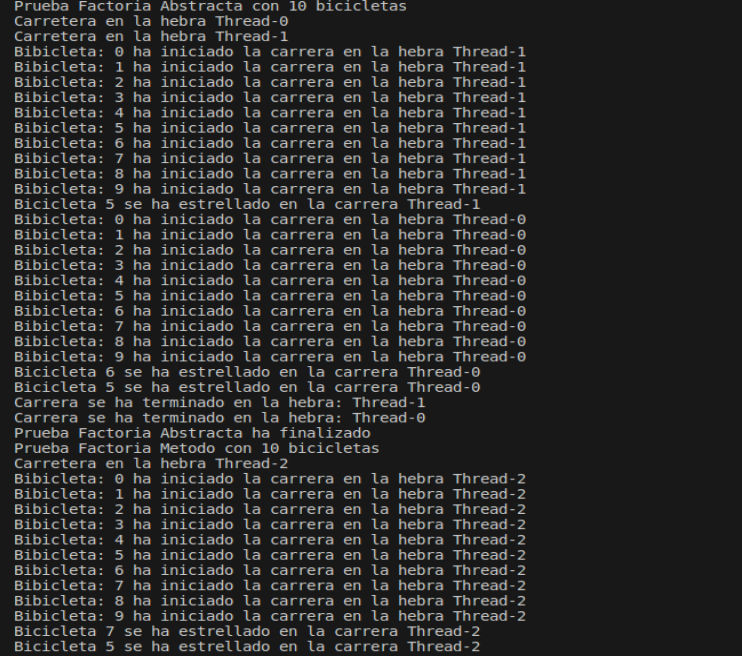
\includegraphics[width=0.8\textwidth]{DS_ejecucion_ej1-1.png}
        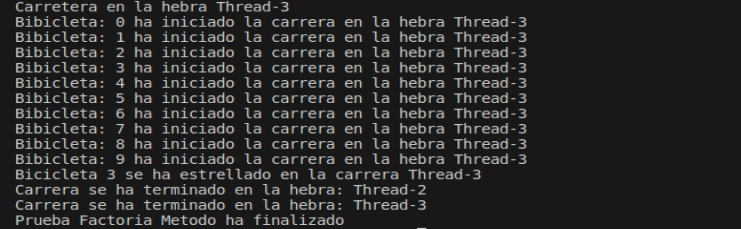
\includegraphics[width=0.8\textwidth]{DS_ejecucion_ej1-2.png}
	\caption{Ejecucion del ejercicio 1}
	\label{fig:ej1}
\end{figure}



\newpage
\section{Ejercicio 2}
\subsection{Análisis}
En este problema se pide realizar la implementación de Factoria Abstracta del ejercicio 1 en el lenguaje Python sin utilizar las hebras y además realizar la implementación del patron \textit{Prototipo}. 

\subsection{Factoria Abstracta}
Utilizamos el modulo \textit{abc} para poder definir clases abstractas. Las clases abstractas son clases que no pueden ser instanciadas directamente, sino que se utilizan como base para otras clases que las heredan. 
El planteamiento no cambia en absolutamente nada en comparación con el ejercicio 1 siendo la única diferencia el lenguaje de programación y su sintaxis subyacente.

\subsection{Prototipo}
Este patrón consiste en crear nuevos objetos clonando otro existente. En nuestro caso vamos a definir un método para la entidad \textit{Bicicleta} que nos permita realizar una copia del objeto existente. Puesto que hablamos de copiar los objetos es necesario recordar los conceptos \textit{shallow copy y deep copy}. 

\begin{itemize}
	\item \textit{Shadow Copy}  copia solo la estructura  del objeto pero comparte los datos miembros entre el original y la copia, lo que hace que los cambios afecten a ambos. Es más rápida y consume menos memoria.
	
	\item \textit{Deep Copy }crea copias independientes evitando la compartición de memoria por tanto los cambios en una copia no afectan al objeto original ni viceversa. Es más lenta y consume más memoria.
\end{itemize}

Para implementar metodo \textit{clone()} podemos recurir al \textit{constructor de copia} en el que realizaremos una copia profunda del objeto recibido como argumento. O alternativamente podemos usar modulo \textit{copy} que nos dá interfaces para duplicar los objetos. Nosotros hemos optado por este último.


\subsection{Ejecución}
\begin{figure}[h]
	\centering
        \vspace{5pt}
	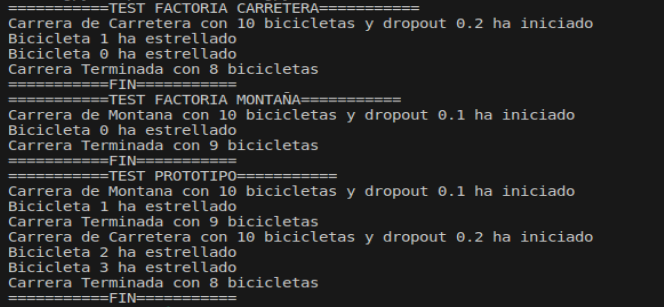
\includegraphics[width=0.8\textwidth]{DS_ejecucion_ej2.png}
	\caption{Ejecucion del ejercicio 2}
	\label{fig:ej2}
\end{figure}



\newpage
\section{Ejercicio 3}
\subsection{Análisis}
En este ejercicio se propone realizar diseño e implementación de una aplicación que utilice un patrón de diseño libre. Para realización de este ejercicios proponemos el siguiente enunciado: 

\vspace{\baselineskip}

\emph{La compañía de un prestigioso juego de rol nos ha encargado crear un programa sencillo que permita a los usuarios crear y
visualizar los atributos de los personajes iniciales que pueden crear.}

\vspace{\baselineskip}

Cada personaje tendrá los siguientes atributos:

\begin{itemize}[leftmargin=1cm]
\item \textbf{Primarios:}
Cada atributo primario es un valor numerico positivo, y su suma sera igual a 56.
Los valores de cada atributo primario cambiaran dependiendo de la raza elegida para el personaje
	\begin{itemize}
		\item Fuerza
		\item Destreza
		\item Resistencia
		\item Inteligencia
		\item Sabiduria
		\item Carisma
		\item Percepcion
	\end{itemize}

\item \textbf{Secundarios:}
Cada atributo secundario se calculara segun las operaciones anteriores, las cuales vendran modificadas por la clase
del personaje
	\begin{itemize}
		\item Vida		  	(Resistencia + fuerza)
		\item Stamina	  	(Destreza + Resistencia)
		\item Mana		  	(Inteligencia + Sabiduria)
		\item Persuasion   	(Carisma + Sabiduria)
		\item Agilidad	  	(Destreza + Inteligencia)
		\item Intimidacion 	(Fuerza + Carisma)
		\item Critico		(Percepcion + Inteligencia)
		\item Punteria		(Destreza + Percepcion)
	\end{itemize}

\item \textbf{Nombre}
\item \textbf{Raza}
	\begin{itemize}
		\item Humano
		\item Orco
		\item Elfo
		\item Enano
	\end{itemize}
\item \textbf{Clase}
	\begin{itemize}
		\item Caballero
		\item Ladron
		\item Mago
		\item Ranger
	\end{itemize}
\end{itemize}


Se pide que aquellas clases del programa que solo se usen una vez sean únicas y que se evite instanciar de mas.
También se pide que las funciones para preguntar al usuario y las funciones de creación de personajes estén separadas.

\subsection{UML}

\begin{figure}[H]
	\centering
        \vspace{15pt}
	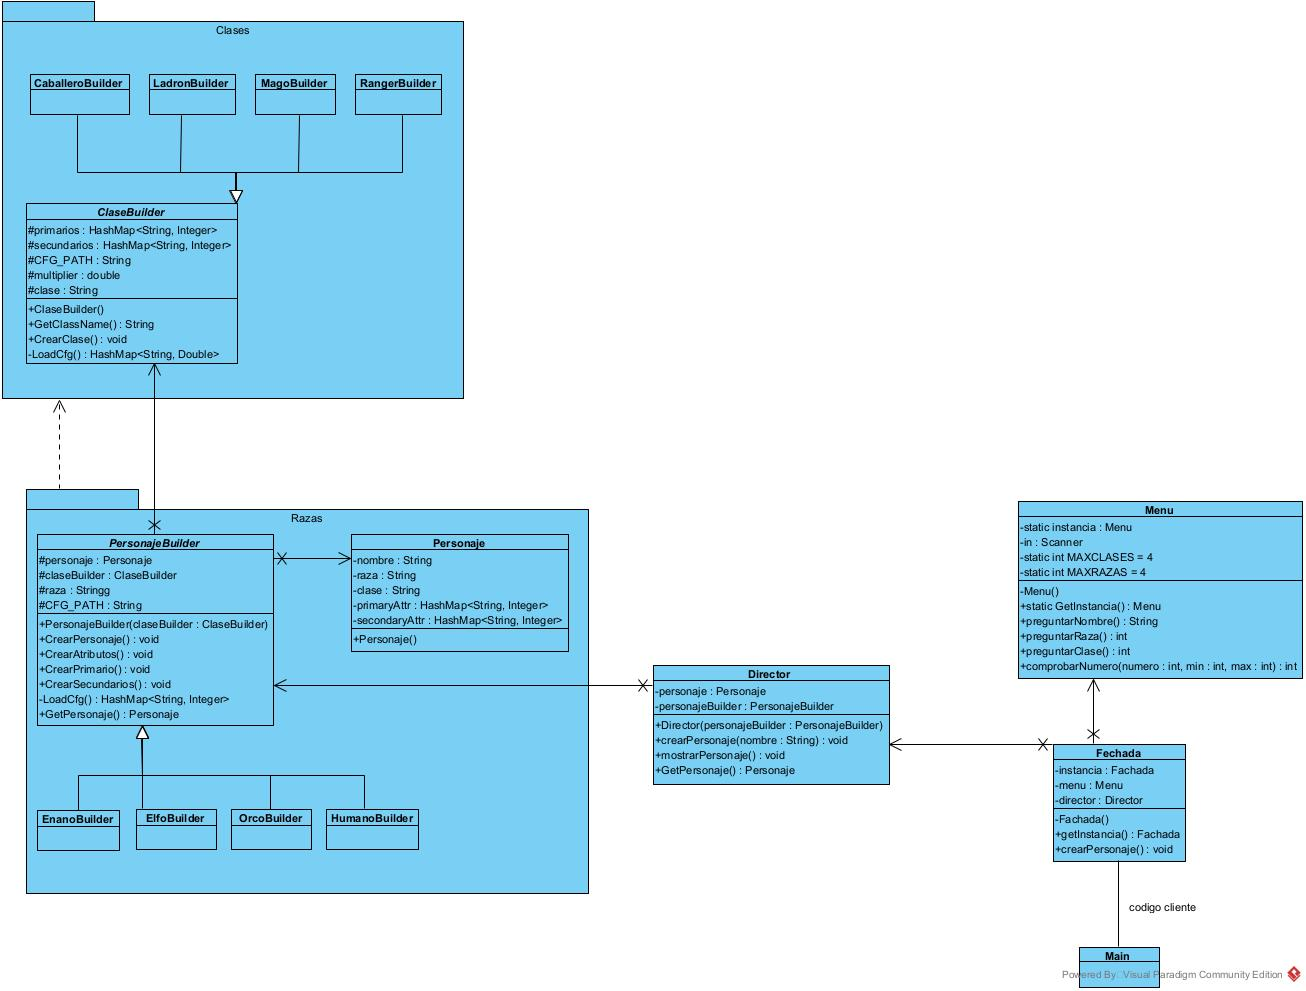
\includegraphics[width=0.9\textwidth]{DS_ej3.jpg}
	\caption{ejercicio 3}
	\label{fig:ej3}
\end{figure}


\subsection{Consideraciones}
\begin{enumerate}[label=-] % Configura la etiqueta de la enumeración como guiones
    \item La clase \textit{ClaseBuilder} es una clase abstracta que actúa como base para las clases hijas. De modo que hemos optado por dar una 
    funcionalidad predeterminada a los métodos para encapsular un comportamiento común y evitar repetir el mismo código en diferentes 
    archivos. De ser necesario una modificación consideramos que es adecuado que cada clase hija mediante override especialice su 
    comportamiento.

    \item Mismo razonamiento se ha aplicado a \textit{PersonajeBuilder}
    
    \item Utilizamos clase \textit{Director} para abstraer el proceso de creación del personaje, es decir, esta clase se encarga de orquestar los pasos necesarior para construir el objeto de tipo \textit{Personaje}.

    \item Utilizamos \textit{Menu} para recoger el input del usuario. Se trata de un \textit{Singleton} pues pensamos que al interactuar a traves de la terminal no tiene sentido que existan muchos objetos de \textit{Menu} instaciados.

    \item Por último, utilizamos clase \textit{Fachada} ofrecemos una interfaz unificada para la interacción con el sistema. De esta forma simplificamos el uso de las clases por el código cliente.

    \item  Como conslución, hemos obtenido un sistema con bajo nivel de acoplamiento. Cada módulo es responsable de una tarea especifica con su lógica adecuada
\end{enumerate}


\newpage
\subsection{Ejecución}
La aplicación le preguntará al usuario por el nombre del personaje, y le permitirá escoger qué raza y clase quiere ser.
Tras obtener respuesta, el programa deberá crear el personaje según los parametros elegidos, y mostrar por pantalla el valor
el nombre del personaje, su raza y su clase, al igual que todos sus atributos con su valor.

\begin{figure}[h]
	\centering
        \vspace{15pt}
	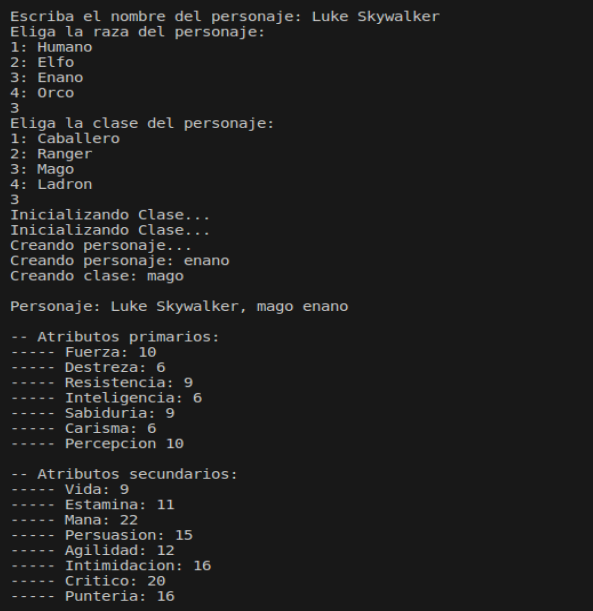
\includegraphics[width=0.75\textwidth]{DS_ejecucion_ej3.png}
	\caption{Ejecucion del ejercicio 3}
	\label{fig:ejecucion_ej3}
\end{figure}

\newpage
\section{Ejercicio 4}
\subsection{Analyse}
In this exercise we had to program a simulator of an engine based on the revolutions per minute (RPM). The imposed model to use for this execise is the Intercepting filter model (filtros de intercepción) which will be further explained in the UML & Flowchart chapter. 
\vspace{15pt}
\item \textbf{The program should have an Graphical interface (GUI):} 
\item One interactive window with the possibility to
\begin{itemize}
   
\item start/stop the engine 
\item start/stop accelerating 
\item start/stop braking;
\end{itemize}
 \item One window which updates in real time 
 \begin{itemize}
     \item RPM 
     \item total kilometres driven 
     \item kilometers driven since the last engine start 
     \item current speed in km/h
 \end{itemize}
 
\subsection{UML and Flowchart}
\begin{figure}[H]
	\centering
        \vspace{15pt}
	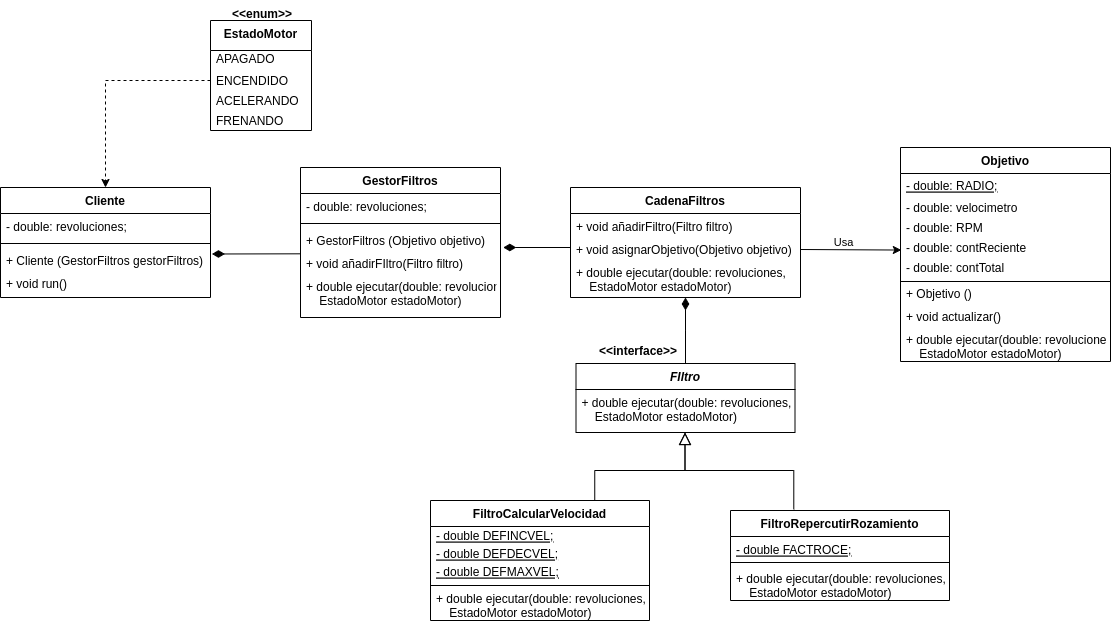
\includegraphics[width=0.9\textwidth]{Ej4.png}
	\caption{ejercicio 4}
	\label{fig:ej4}
\end{figure}

\item The intercepting filter model is best explained using the flowchart (Figure 8). The heart & brain of the program is the "Gestor Filtros". It gets called by the client which in our case is the GUI with the buttons Start/stop, accelerate and break. The GestorFiltro in our case simulates the engine but also creates the object of the class CadenaFiltros and adds the needed Filters to the array in the CadenaFiltros object. The filters are xused to give constraints to the command we want to execute. In our case we have two filters one adding/decreasing rpm and one that calculates the friction. The filters return their values to the object CadenaFiltro and after all filters are applied the values go back to GestorFiltro which sends it to the Objetivo which is in our case the Salpicadero where our computed value can be printed on the window.

\begin{figure}[H]
	\centering
        \vspace{15pt}
	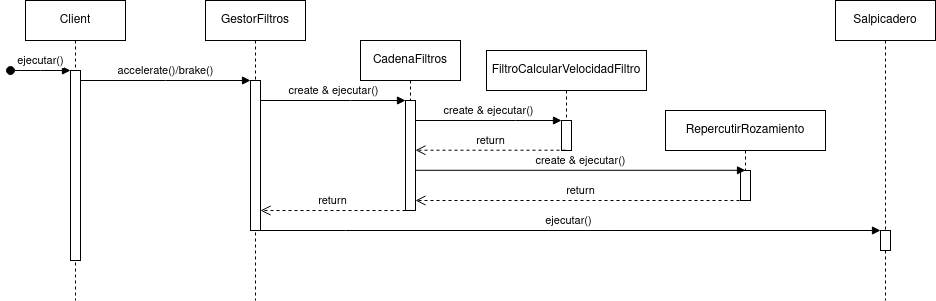
\includegraphics[width=0.9\textwidth]{Flow_EJ4.png}
	\caption{ejercicio 4 Flowchart}
	\label{fig:ej4}
\end{figure}

\subsection{Considerations}
There were 3 main considerations made during the conception of the program
\begin{itemize}
   
\item 1. The engine\\
The question was where to put the code for the engine. We decided putting it in the GestorFiltros and it get's logically called when the Encender button is activated
\item 2. Update frequency\\
We decided updating the rpms (Increasing or decreasing the rpm) every second. 
\item 3. Problem running engine and user interface simultaneously\\
We encountered the problem in the devolopement that if we run the GUI and the engine on the same process they block each other so the engine isn't operable (buttons can't be pushed) when the engine is running
\end{itemize}

\subsection{Execution}
When the program is started two windows open:
\begin{itemize}
    \item An interactive window where you choose your action
    \item A non interactive window where the actual informations are shown
\end{itemize}
\begin{figure}[h]
	\centering
        \vspace{15pt}
	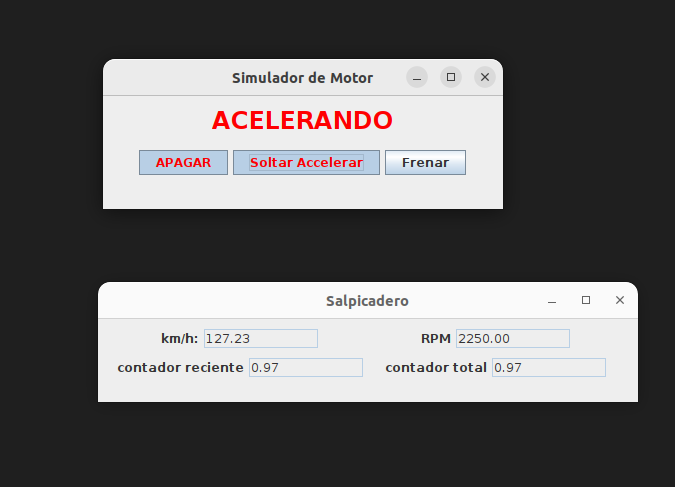
\includegraphics[width=0.8\textwidth]{exec_ej4.png}
	\caption{Ejecucion del ejercicio 4}
	\label{fig:ej4}
\end{figure}


\newpage
\section{Ejercicio 5}
\subsection{Análisis}
En este problema se pide diseñar y realizar una aplicación de WebScraping en Python donde se utilice el Patrón \textit{Strategy} para scrapear
información en vivo de acciones.  Para ello se seguirán dos estrategias cada una usando una biblioteca distinta de Python: BeautifulSoup y Selenium.

\subsection{Strategy}
El patrón \textit{Strategy} o \textit{Estrategia} define una familia de algoritmos, encapsula cada uno y los hace intercambiables en tiempo de
ejecución. Para ello definimos una clase abstracta llamada \textit{ScraperStrategy} y las estategias de scrapping correspondientes
\textit{BeautifulSoupScraper} y \textit{SeleniumScraper}. Además, es necesario crear un clase que sirva para intercambiar las estrategias
definidas en cada ejecución, sirviendo para esto la clase \textit{Context}.

\begin{figure}[h]
	\centering
        \vspace{15pt}
	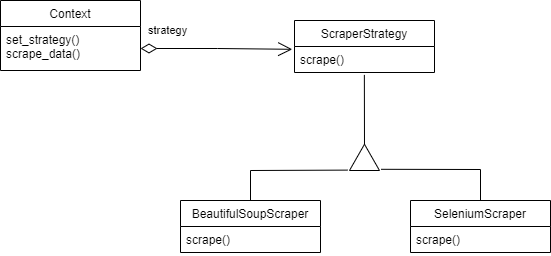
\includegraphics[width=0.6\textwidth]{DS_ej5.drawio.png}
	\caption{Strategy}
	\label{fig:strategy}
\end{figure}


\subsection{Solución}
Horadando en el código de cada estrategia de scrapping, \textit{SeleniumScraper} ha supuesto un ejercicio de mayor complejidad. Al intentar llevar a cabo este algoritmo, en primera instancia, obteníamos
errores debido a la ventana emergente que informa de las cookies nada más entrar en la web. Para sortearla, es necesario pulsar sobre cualquiera de
los botones de \textit{Aceptar} o \textit{Rechazar}, sin embargo, estos botones son visibles únicamente si la pantalla cumple unas propiedades 
específicas de tamaño, si no, es necesario realizar un scroll vertical para alcanzar dichos botones. La solución planteada a esta tesitura ha sido 
primero maximizar la ventana, garantizando así la visibilidad de los botones, para luego pulsar sobre el botón de \textit{Rechazar} y finalmente 
acceder a los datos que queremos obtener. Utilizando \textit{BeautifulSoup} ha sido necesario hacer únicamente esta útlima parte.


\subsection{Ejecución}
Durante la ejecución debemos ingresar el símbolo de la acción, y luego seleccionar un método de scrapping: 1 para \textit{BeautifulSoup} y 
2 para \textit{Selenium}. Finalemente, esto nos permitirá guardar los datos que queríamos alamcenar en el documento url\textunderscore{}info.json.

\begin{figure}[h]
	\centering
        \vspace{15pt}
	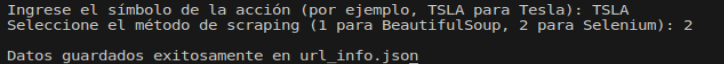
\includegraphics[width=0.8\textwidth]{DS_ejecucion_ej5-1.png}
	\caption{Ejecucion del ejercicio 5}
	\label{fig:ej5}
\end{figure}

\newpage
\begin{figure}[h]
	\centering
        \vspace{15pt}
        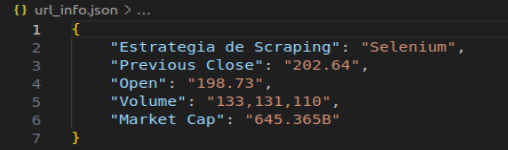
\includegraphics[width=0.6\textwidth]{DS_ejecucion_ej5-2.png}
	\caption{Archivo resultante de la ejecución del ejercicio 5}
	\label{fig:archivo_ej5}
\end{figure}



\end{document} 